\section{QPSK Transmitter}

\begin{refsection}

--------------------------------------------------------------------\\
2017-08-25, \underline{Review}, Armando Nolasco Pinto\\
--------------------------------------------------------------------\\

This system simulates a QPSK transmitter~\cite{loudon2000}. A schematic representation of this system is shown in figure \ref{QPSK_transmitter_block_diagram_simple}.

\begin{figure}[h]
	\centering
	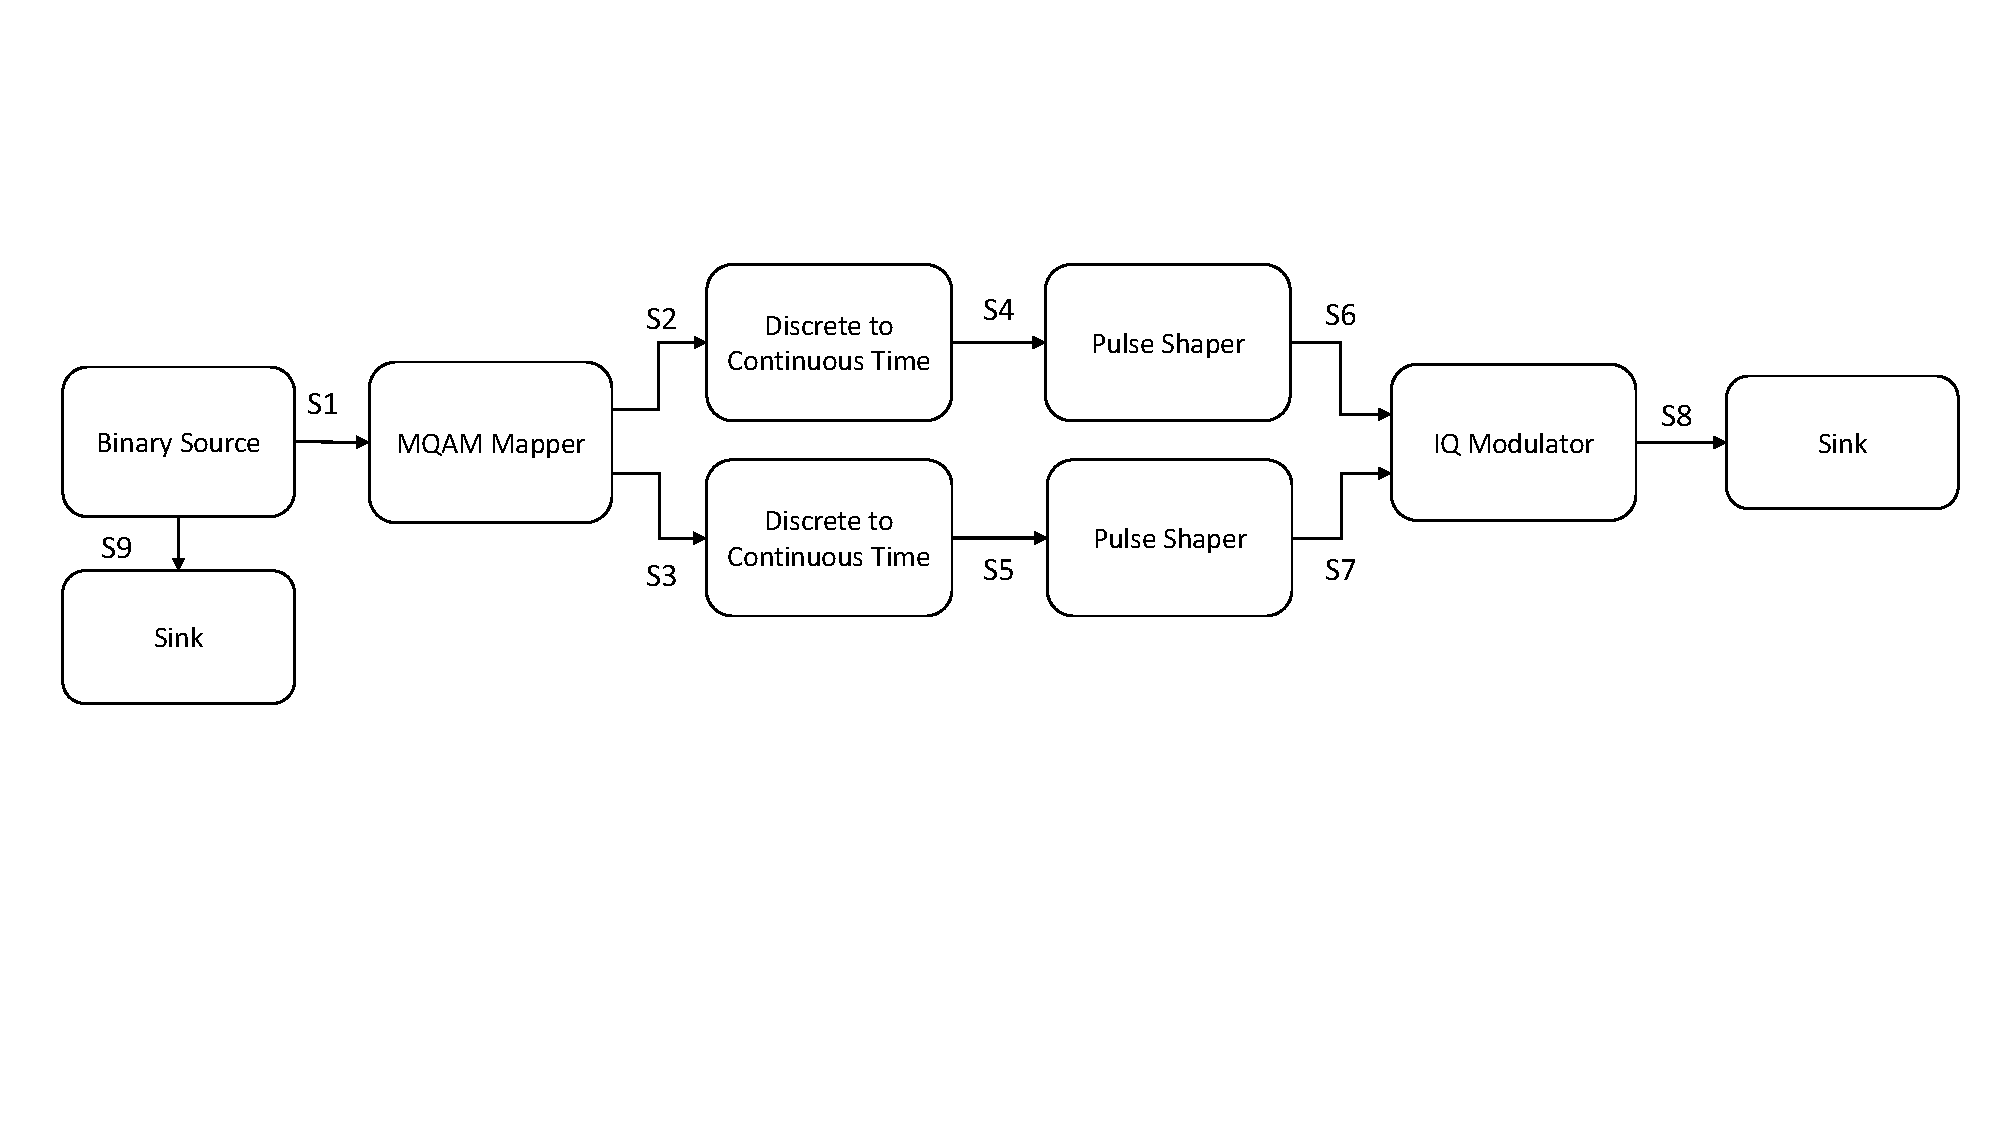
\includegraphics[width=1.0\textwidth]{./sdf/qpsk_transmitter/figures/qpsk_transmitter.pdf}
	\caption{QPSK transmitter block diagram.}\label{QPSK_transmitter_block_diagram_simple}
\end{figure}

\subsection*{System Input Parameters}
\hspace{10mm}
\renewcommand{\labelitemi}{\textbf{Parameter: }}
\renewcommand\labelitemii{\textbf{Description: }}
\renewcommand\labelitemiii{\textbf{Accepted Values: }}
 \begin{itemize}

   \item  \emph{sourceMode}
   \begin{itemize}
     \item  Specifies the operation mode of the binary source.
     \begin{itemize}
       \item  PseudoRandom, Random, DeterministicAppendZeros, DeterministicCyclic.
     \end{itemize}
   \end{itemize}

   \item  \emph{patternLength}
   \begin{itemize}
     \item  Specifies the pattern length used my the source in the PseudoRandom mode.
     \begin{itemize}
       \item  Integer between 1 and 32.
     \end{itemize}
   \end{itemize}

    \item  \emph{bitStream}
   \begin{itemize}
     \item  Specifies the bit stream generated by the source in the DeterministicCyclic and DeterministicAppendZeros mode.
     \begin{itemize}
       \item  "XXX..", where X is 0 or 1.
     \end{itemize}
   \end{itemize}

    \item  \emph{bitPeriod}
   \begin{itemize}
     \item  Specifies the bit period, i.e. the inverse of the bit-rate.
     \begin{itemize}
       \item  Any positive real value.
     \end{itemize}
   \end{itemize}

   \item  \emph{iqAmplitudes}
   \begin{itemize}
     \item  Specifies the IQ amplitudes.
     \begin{itemize}
       \item Any four par of real values, for instance \{ \{ 1,1 \},\{ -1,1 \},\{ -1,-1 \},\{ 1,-1 \} \}, the first value correspond to the "00", the second to the "01", the third to the "10" and the forth to the "11".
     \end{itemize}
   \end{itemize}

   \item  \emph{numberOfBits}
   \begin{itemize}
     \item  Specifies the number of bits generated by the binary source.
     \begin{itemize}
       \item Any positive integer value.
     \end{itemize}
   \end{itemize}

     \item  \emph{numberOfSamplesPerSymbol}
   \begin{itemize}
     \item  Specifies the number of samples per symbol.
     \begin{itemize}
       \item Any positive integer value.
     \end{itemize}
   \end{itemize}

   \item  \emph{rollOffFactor}
   \begin{itemize}
     \item  Specifies the roll off factor in the raised-cosine filter.
     \begin{itemize}
       \item A real value between 0 and 1.
     \end{itemize}
   \end{itemize}

      \item  \emph{impulseResponseTimeLength}
   \begin{itemize}
     \item  Specifies the impulse response window time width in symbol periods.
     \begin{itemize}
       \item Any positive integer value.
     \end{itemize}
   \end{itemize}

 \end{itemize}


% bibliographic references for the section ----------------------------
\clearpage
\printbibliography[heading=subbibliography]
\end{refsection}
\addcontentsline{toc}{subsection}{Bibliography}
\cleardoublepage
% --------------------------------------------------------------------- 